\section{Introduction}
\label{sec:introduction}

\begin{figure}[t]
  \centering
%   \fbox{\rule{0pt}{2in} \rule{0.9\linewidth}{0pt}}
   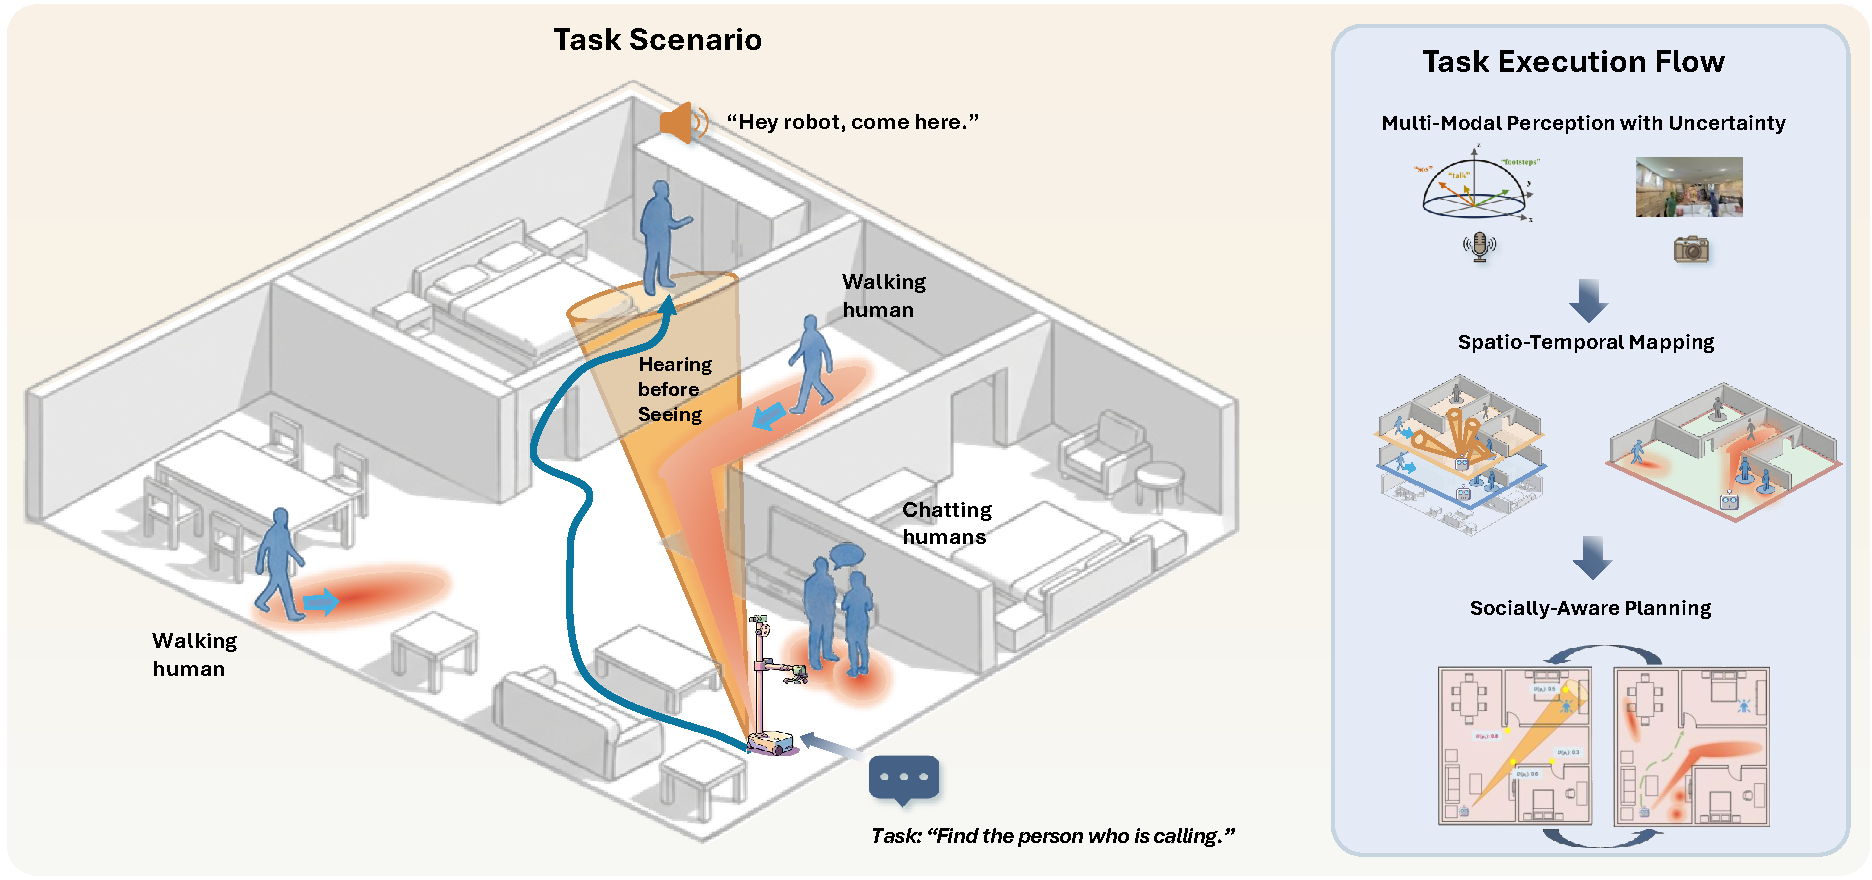
\includegraphics[width=\linewidth]{figures/teaser}
   \caption{\textbf{SAVNav Overview.} (Left) \textit{Task Scenario:} The robot receives a natural language instruction and navigates to a target (e.g., "Person seeking help") while avoiding humans. Crucially, the system handles Non-Line-of-Sight (NLOS) risks by detecting the acoustic Direction of Arrival (orange cone) of unseen walking humans. This allows the planner to anticipate potential collisions and adjust the path (blue curve) proactively. (Right) \textit{Execution Flow:} Our framework processes instructions and fuses visual observations with uncertainty-aware acoustic perception to build a spatio-temporal map for socially-aware planning.}
   \label{fig:teaser}
\end{figure}

As mobile robots increasingly transition from controlled industrial environments to shared human spaces, such as homes and offices, the requirement for navigation shifts from collision-free efficiency to social compliance. Social navigation requires robots to respect human comfort, maintain appropriate distances, and adhere to social norms \cite{social_nav_survey}. While significant progress has been made in modeling human-robot interaction, current systems often fail in highly dynamic, unstructured environments where safety is paramount.

A critical limitation of existing social navigation frameworks is their heavy reliance on vision. Visual sensors are inherently limited to Line-of-Sight (LOS) perception. They are susceptible to field-of-view constraints and physical occlusions, rendering robots blind to dynamic risks emerging from behind corners or obstacles. This limitation frequently leads to the ``corner surprise'' problem, where a robot must execute an unsafe emergency stop upon suddenly detecting a pedestrian. In contrast, humans naturally leverage audio---a modality with omnidirectional and diffractive properties---to perceive Non-Line-of-Sight (NLOS) risks, effectively ``hearing before seeing.'' Despite this intuitive advantage, the integration of audio for dynamic risk anticipation remains underexplored in robotics.  

This gap exists primarily due to a dichotomy in current research. Audio-Visual Navigation (AV-Nav) typically focuses on locating static sound sources (e.g., a ringing phone) \cite{av_nav_survey}, ignoring the social implications of sound as a dynamic movement cue. Conversely, Social Navigation focuses on avoidance but neglects the acoustic modality. Bridging this gap has been hindered by the lack of unified simulation infrastructure; high-fidelity acoustic simulators (e.g., SoundSpaces \cite{soundspaces}) often lack the dynamic human agents found in social navigation platforms (e.g., Habitat-Lab \cite{habitat}). Consequently, there is no standardized testbed for developing agents that can navigate using the acoustic footprint of moving humans.

To address these challenges, we introduce \textbf{SAVNav} (Socially-Aware Audio-Visual Navigation), a framework that unifies high-fidelity acoustics with dynamic social agents. Our system goes beyond simple multi-modal fusion; it fundamentally treats sound as a predictor of future visual occupancy. We introduce the concept of \textit{Acoustic Hallucinated Momentum}, where the robot projects a virtual risk field into NLOS regions based on acoustic Direction of Arrival (DoA), forcing the planner to anticipate potential collisions before visual confirmation. Furthermore, to handle the inherent ambiguity of sound, we propose an information-theoretic \textit{Active Search} mechanism that guides the robot to viewpoints that maximize information gain, resolving perceptual uncertainty proactively.

Our main contributions are as follows:
\begin{itemize}
    \item \textbf{Infrastructure \& Task:} We develop the first unified simulation platform integrating physical acoustics (SoundSpaces 2.0) with dynamic human agents (Habitat-Lab 3.0), defining the novel SAVNav task and benchmark.
    \item \textbf{Uncertainty-Aware Methodology:} We propose a modular navigation framework that introduces \textit{Hallucinated Momentum} for NLOS risk anticipation and an \textit{Information-Theoretic Active Search} strategy to resolve perceptual ambiguity using negative visual information.
    \item \textbf{System Validation:} We demonstrate a complete Sim-to-Real deployment on a Stretch 3 mobile manipulator. Our system exhibits robustness to real-world reverberation and background noise, effectively mitigating blind-corner collisions where vision-only baselines fail.
\end{itemize}
